\documentclass[UTF8,a4paper,11pt]{article}
% \usepackage[UTF8]{ctex}

\usepackage{CJKutf8} %支持中文
\usepackage[T1]{fontenc}
\usepackage[utf8]{inputenc}
% \usepackage{unicode-math}
\usepackage{lmodern}
\usepackage{listings}
\usepackage{amsmath} %提供\begin{equation}
\usepackage{amssymb} %提供\substack
\usepackage{latexsym}
\usepackage{cite}
\usepackage{bm} %在需要加粗的数学公式前使用\bm命令
% \usepackage{tabularx}
% \usepackage{dcolumn}

\title{小学五年级数学(上) }
\author{俞书心}

% begin 选择题选项排版
\usepackage{lipsum}
\usepackage{enumitem}
\usepackage{tikz} %
\usepackage{graphicx}%以下代码不依赖宏包,加它纯粹为演示图形选项
%预备
\newlength\lxxmax
\newlength\lhalf
\newlength\lhalfhalf
\newsavebox\xxboxa
\newsavebox\xxboxb
\newsavebox\xxboxc
\newsavebox\xxboxd
\newcommand\getboxsandmax[4]{%存放内容并获取最大宽
\sbox\xxboxa{#1}%
\sbox\xxboxb{#2}%
\sbox\xxboxc{#3}%
\sbox\xxboxd{#4}%
\ifdim\wd\xxboxa>\wd\xxboxb
\lxxmax\wd\xxboxa\relax
\else
\lxxmax\wd\xxboxb\relax
\fi
\ifdim\lxxmax<\wd\xxboxc
\lxxmax\wd\xxboxc\relax
\fi
\ifdim\lxxmax<\wd\xxboxd
\lxxmax\wd\xxboxd\relax
\fi
}


%四选项自动排版,用法 \xx{选项}{选项}{选项}{选项}
\newcommand\xx[4]{\par
\getboxsandmax{A. #1}{B. #2}{C. #3}{D. #4}%
\addtolength\lxxmax{1em}%
\setlength\lhalf{\dimexpr(\linewidth-\parindent)/2\relax}%
\setlength\lhalfhalf{.5\lhalf}%
\ifdim\lxxmax>\lhalf
    A. #1 \par
    B. #2 \par
    C. #3 \par
    D. #4
\else
    \ifdim\lxxmax>\lhalfhalf
        \begin{minipage}{\lhalf}
        \usebox\xxboxa
        \end{minipage}%
        \begin{minipage}{\lhalf}
        \usebox\xxboxb
        \end{minipage}\par
        \begin{minipage}{\lhalf}
        \usebox\xxboxc
        \end{minipage}%
        \begin{minipage}{\lhalf}
        \usebox\xxboxd
        \end{minipage}%
    \else
        \begin{minipage}{\lhalfhalf}
        \usebox\xxboxa
        \end{minipage}%
        \begin{minipage}{\lhalfhalf}
        \usebox\xxboxb
        \end{minipage}%
        \begin{minipage}{\lhalfhalf}
        \usebox\xxboxc
        \end{minipage}%
        \begin{minipage}{\lhalfhalf}
        \usebox\xxboxd
        \end{minipage}%
    \fi
\fi
}

%四图片选项专用(每图不得太宽)
\newcommand\fourtuxx[4]{\par\vspace{2ex}%
\getboxsandmax{#1}{#2}{#3}{#4}%
\addtolength\lxxmax{1em}%
\setlength\lhalf{.5\linewidth}%
\setlength\lhalfhalf{.5\lhalf}%
\ifdim\lxxmax>\lhalf
images too big! please change width to less than 0.5linewidth-1em.
\else
    \ifdim\lxxmax>\lhalfhalf
        \noindent
        \begin{minipage}[b]{\lhalf}
        \centering
        \usebox\xxboxa\par A
        \end{minipage}%
        \begin{minipage}[b]{\lhalf}
        \centering
        \usebox\xxboxb\par B
        \end{minipage}\par\vspace{2ex}%
        \noindent
        \begin{minipage}[b]{\lhalf}
        \centering
        \usebox\xxboxc\par C
        \end{minipage}%
        \begin{minipage}[b]{\lhalf}
        \centering
        \usebox\xxboxd\par D
        \end{minipage}%
    \else
        \noindent
        \begin{minipage}[b]{\lhalfhalf}
        \centering
        \usebox\xxboxa\par A
        \end{minipage}%
        \begin{minipage}[b]{\lhalfhalf}
        \centering
        \usebox\xxboxb\par B
        \end{minipage}%
        \begin{minipage}[b]{\lhalfhalf}
        \centering
        \usebox\xxboxc\par C
        \end{minipage}%
        \begin{minipage}[b]{\lhalfhalf}
        \centering
        \usebox\xxboxd\par D
        \end{minipage}%
    \fi
\fi
}
%end 选择题选项排版

% 正文区
\begin{document}
% \begin{CJK}{UTF8}{gkai}
\begin{CJK}{UTF8}{gbsn}
\maketitle
\tableofcontents

\begin{abstract}
小学数学易错题汇总
\end{abstract}

\newpage
\section{填空题}

% 自定义列表序号
\makeatletter 
\def\zdyxh#1{\expandafter\@zdyxh\csname c@#1\endcsname} 
\def\@zdyxh#1{% 
\ifcase#1\or 1\or 2\or 3\or 4\or 5\or 6\or 7\or 8\or 9\or 10\or 11\or 12\or 13\or 14\or 15\or 16\else 超了\fi} 
\makeatother 
\AddEnumerateCounter*{\zdyxh}{\@zdyxh}{1} 
% 没搞懂下面这句是干啥用的
% \lipsum[101]
\begin{enumerate}[label=\zdyxh*.] 
\item \begin{math}
 7.8\div1.6\ (\qquad  )\ 78 \div16 
\end{math}
\item $145.6\div 4 = \underline{\qquad}$
\item $49\mbox{克}= (\qquad )\mbox{千克} \qquad 0.28\mbox{千克}=(  \qquad)\mbox{克} \qquad 12cm^2=( \qquad)dm^2 $
\item $\dfrac{1}{2}=1\underline{\qquad     }2$
\item 45分钟=\underline{\qquad     }时
\item $1.32m^2=\underline{\qquad     }dm^2 $
\item 一个四位小数用四舍五入法保留两位小数是5.047,这个四位小数最大是\underline{\qquad\qquad },最小是\underline{\qquad\qquad },最大和最小差是\underline{\qquad\qquad }。 
\item 内容 
\item 内容 
\item 内容
\item 内容

%\lipsum[101] 
\end{enumerate}


\section{选择题}



\section{计算题(除不尽的保留两位小数)}
 $0.62\div3.1=$ \qquad\qquad $37.12\times6.4\approx $\\
竖式计算\\
$30.1\div 33\approx $ \qquad\qquad $17.4\div1.6\approx$
\\ \\ \\ \\ \\ 

武汉$\rightarrow$蔡甸128公里,武汉$\rightarrow$孝感192公里,孝感$\rightarrow$蔡甸156公里,小明开车从蔡甸到武汉用了1小时36分钟,小明开车从武汉到孝感要多少小时?(用两种方式以上计算)
\\ \\ \\ \\ \\ \\

爸爸带了12000元人民币去银行兑换日元,能兑换多少日元?(每100日元兑换人民币6.15元)
\\ \\ \\ \\ \\ \\

\section{问答题}
\begin{tabular}{lr}
&12\\
+&143\\
+&654\\
+&24\\
\hline
=&\small$\square\!\square\!\square$ \\ \\
\end{tabular}

% $\polylongdiv{25.3}{23}$


这是一张小胖家今年6月的电费帐单,有些数据看不清楚,你能根据我们学的知识把它补完整吗? \\ 
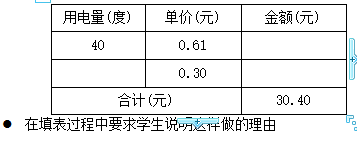
\includegraphics{./pic/5-1-1.jpg}

\clearpage % 防止\tableofcontents和section{汉字}共用时编译报错
\end{CJK}
% \newpage
\end{document}
